\graphicspath{{chapters/analysis/images/}}
\label{sec:fitting_data}
\section{Fitting Data}
Icecube analyses are developed blindly in order to minimize bias.
This proceeds in a few distinct stages, each described separately here.

\unsure{may just remove the burn sample crap. its so out of date that its too weird to go back and redo it.}
\label{subsec:burn_sample}
\subsection{Burn Sample Fits: Testing the Fitting Code}
Analyzers are initially restricted to a small fraction of the full dataset while developing the event selection and fitting codes.
The size of the burn sample, here limited to 1\% of the total dataset, is selected in order to provide reasonable statistics while maintaining limited sensitivity to the final physics parameters.
Once end-to-end tests are completed using solely simulated events, this small sample, known as the \textbf{burn sample}, is fit in order to verify that results obtained are reasonable.

\improvement{blahdy blahdy blahdy. no point spending time here if i may just kill it}


\label{subsec:blind_fits}
\subsection{Blind Fits: Checking the Goodness-of-Fit}
Once the burn sample tests are complete, the next stage is to perform what is known as a \textbf{blind fit}.
The concept, developed for oscillation analyses in IceCube, exists as an intermediate stage between the low-sensitivity burn sample tests and the final fit 
Unlike the burn sample fits, the blind fits use the full data sample for testing.
All systematics are included in the fit as normal.
The final physics parameters, in this case the oscillation parameters and the $\nu_\tau$ normalization, are allowed to fit freely, but the final results are obfuscated.
The goodness-of-fit and systematics values are free for investigation.
Analyzers are free to move onto a request for full unblinding if the goodness-of-fit exceeds 5\%.
If the goodness-of-fit is significantly lower than this limit, the sample and fit is investigated further to identify any potential issues or oversights.
The blind fit is a test designed to look for problems prior to full unblinding in order to implement necessary fixes while remaining blind to the effect on the final result.

The goodness-of-fit, known more informally as the p-value associated with the fit, may be calculated via two closely-related methods.
An ensemble of Monte Carlo trials is fit and the resulting $\chi_{FS}^2$ values are used.
The fraction of trials with $\chi_{FS}^2$ larger than that observed in data gives the first p-value.
The second method uses SciPy \findref{scipy} to fit a $\chi^2$ distribution. 
The p-value may then be calculated from the continuous distribution by finding the total probability of observing a fit with a $\chi_{FS}^2$ value equally or worse than the data fit, $\mathtt{P_2\left(\chi_{FS}^2 \geq \left(\chi_{FS}^2\right)_{Data}\right)}$.

The first method generally will yield more accurate results, particularly if the resulting distribution is poorly fit by a simple $\chi^2$ distribution. 
If the fit is particularly poor, a large number of trials may be necessary in order to calculate an accurate p-value.
In these cases, the second method may be used to provide an estimate of the p-value of the fit.

During the first work with blind fits, this analysis used a wide range of reconstructed energies, including events up to 800 GeV in order to better constrain systematics terms in the non-oscillating higher energy regions.
Blind fits in the GRECO analysis initially showed significant disagreement between the data and simulation, with a goodness-of-fit of $\mathtt{10^{-7}}$.
Investigations yielded new discoveries about both the calibration of the Monte Carlo simulation and previously-unknown erroneous events in the data.

\label{subsubsec:charge_templates}
\subsubsection{Disagreement in Charge Templates}
Continuing problems with the goodness-of-fit led to still more unique discoveries using the GRECO sample.
While checking variables, significant disagreement was discovered in numerous charge variables.
A proxy for the most fundamental variable, the average charge per hit DOM, shown in \needfig{q/nch at L7}, shows systematic disagreement between the simulated events and all years of detector data.

The first suspected cause was the erroneous splitting of waveform pulses in the WaveDeform charge extraction module\findref{wavedeform?}.
The expected charge from a single incident photoelectron is used in WaveDeform to convert the digitized waveforms from the FADC and ATWD into reconstructed photoelectrons consisting of charge and timing information.
While the simulated response is known exactly, the associated charge response of the DOM in data requires careful calibration.
Using a mismodeled charge response to extract pulses in the data can result in single photoelectrons being erroneously split into multiple smaller reconstructed pulses.
Potential mismodeling effects of the charge extraction were checked in \ref{fig:pulse_timing_profile}. 
In these figures, the charge of each individual pulse is shown as a function of the arrival time, which is normalized to the time of the largest extracted pulse in the DOM for each event.

\begin{center}
\begin{figure}
	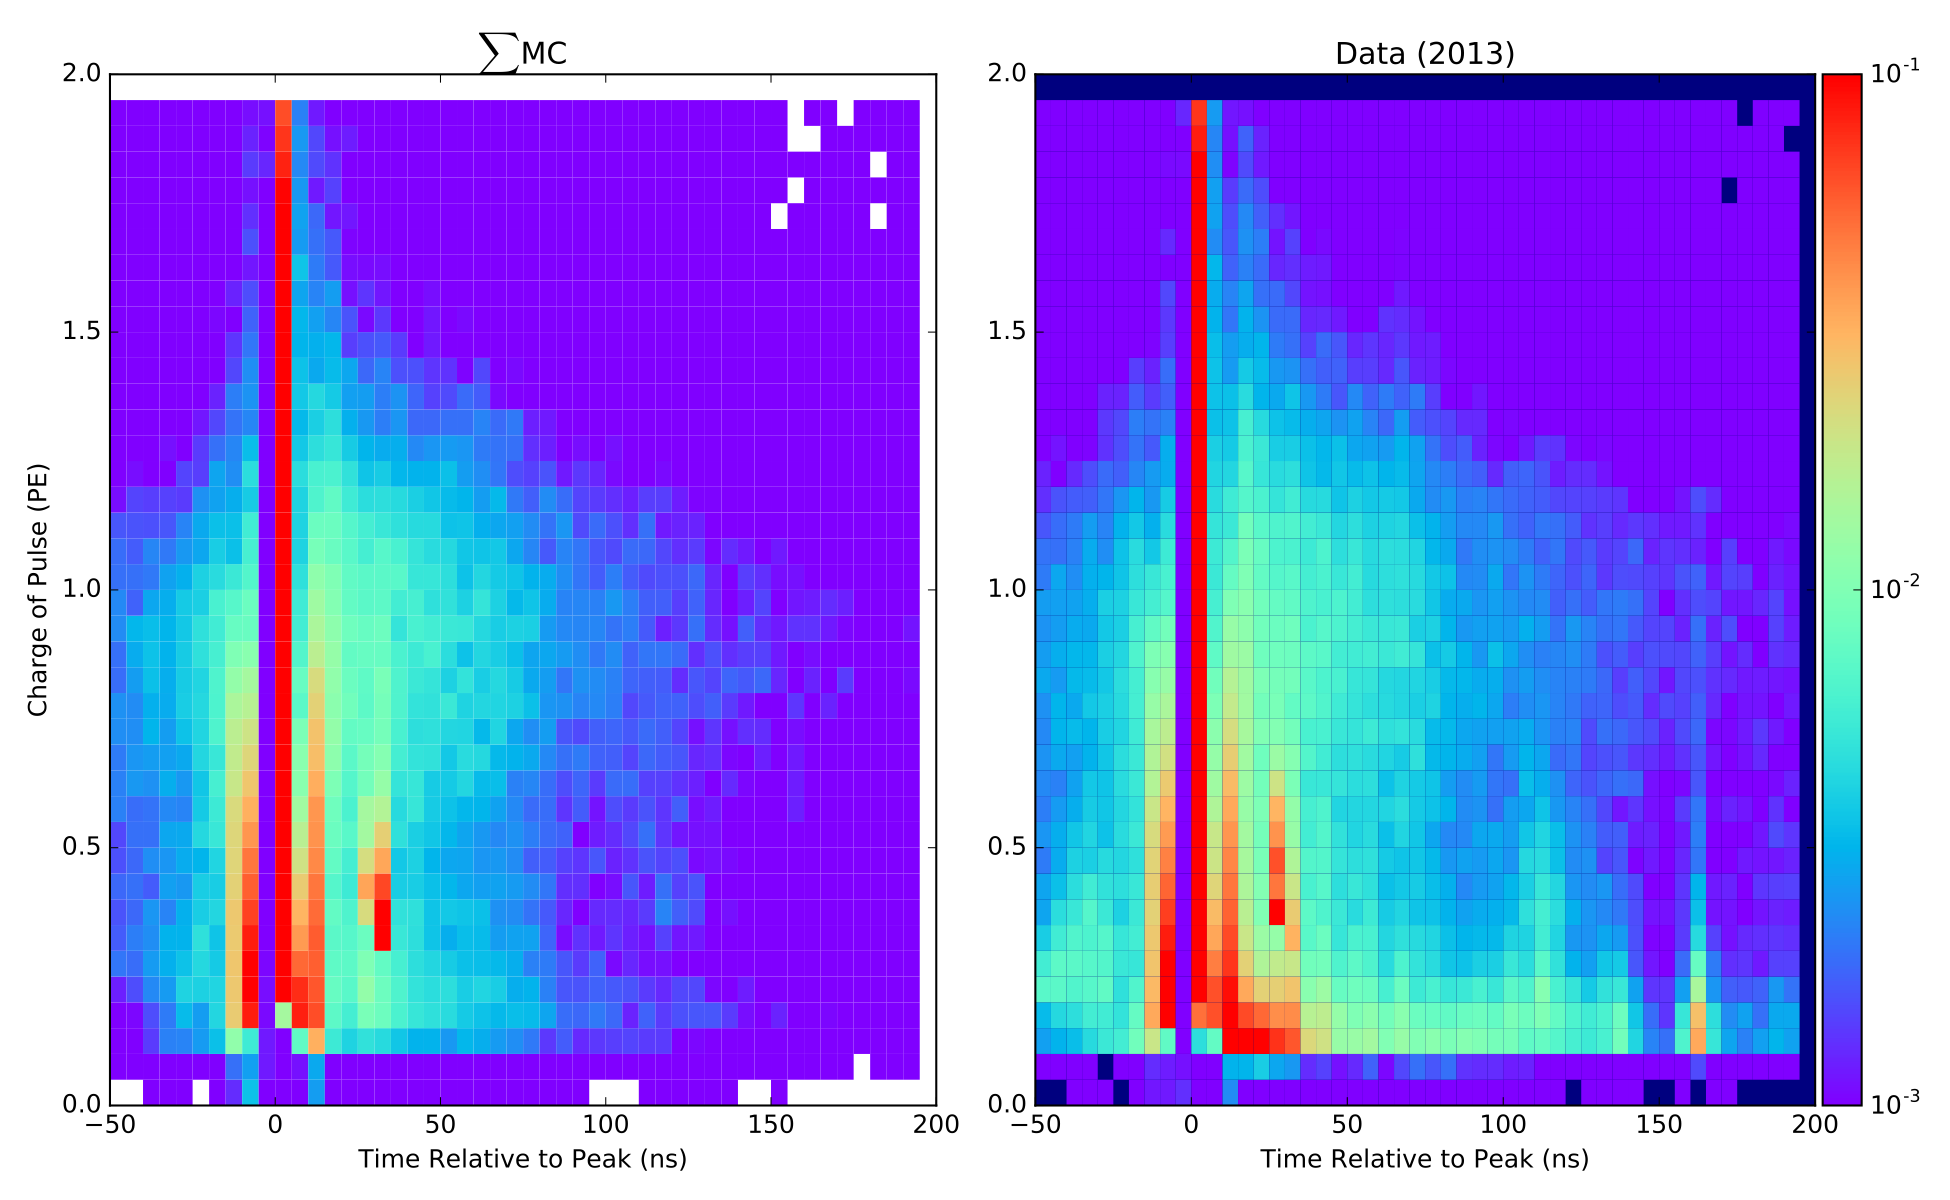
\includegraphics[width=0.9\linewidth]{2d_maps_detail_raw.png}
\label{fig:pulse_timing_profile}
\caption{A comparison of the charge extraction in data and simulation at GRECO L7. Both the time and charge are shown for individual pulses on all DOMs. The time is measured relative to the largest pulse observed on each DOM during an event. The data and simulation histograms are independently normalized to 1.0. While the two show broad agreement, notable differences occur at low charge.}
\end{figure}
\end{center}

Significant disagreements between the data and simulation are visible.
The erroneously split pulses are visible in data as a low-charge tail from t=0 until t=50 nanoseconds.
In addition to this effect, however, many other regions of disagreement are visible.
In data, there appear to be a significant number of prepulses not visible in the simulation occuring between t=-50 and t=-20 nanoseconds.
The structure of the late pulses, appearing with approximately 0.4 PE of charge and at time t=30 nanoseconds also appears notably different between the data and simulation.
A final set of pulses, occuring at 160 nanoseconds, also appears to be unsimulated.
This timing structure requires additional calibration resources to identify and better simulate, the scope of which is beyond this work.
Regardless, the presence of unsimulated features indicates that at least some charge information in the simulation is unreliable.

The absence of features led to investigations of the charge produced in PMTResponseSim module of DOMLauncher.
In the module, photoelectrons at the photocathode of the PMT are propagated through the dynodes to the anode.
The resulting output, a series of pulses emitted from the PMT to be passed onto the simulation of the DOM discriminator and digitization processes, requires a conversion from the number of raw incident photoelectrons to a total charge profile in the form of a waveform.
The conversion, known as the \textbf{single photoelectron template}, or \textbf{SPE template}, is calculated from calibration measurements performed prior to deployment of the DOMs in the ice \findref{TA003 charge template}.
The SPE template, used for all DOMs, has been known to vary somewhat between DOMs in a lab setting for many years, but the problem was deemed unimportant given other ongoing calibration work.

With the identification of the issue using the GRECO event selection, new efforts were dedicated to the production of in-situo measurements of the SPE templates for each DOM.
These new template are entering production as of the time of this analysis, but the time required for newly updated simulation is prohibitive.
Other methods are therefore necessary to avoid introducing spurious systematic biases into the final results.

In order to attempt to characterize the expected effect due to the change in the SPE templates, a new method of reweighting was developed with the GRECO selection.
The average charge per DOM, $\mathtt{\bar{q}}$, is shifted by a known amount, $\mathtt{\Delta \bar{q}}$ and binned.
The ratio of the shifted and unshifted average charge histograms is calculated.
An example of this process for the $\mathtt{\nu_\mu^{CC}}$ is shown in \needfig{example of shifted and unshifted charges for eg numu}.
This process is performed for various values of $\mathtt{\Delta \bar{q}}$ and the resulting ratios are splined using the SciPy splining function RectBivariateSpline \findref{scipy rectbivariatespline}, yielding a continuous function describing the change in the number of events at each charge as a function of $\mathtt{\Delta \bar{q}}$.
This spline, an example of which is shown in \needfig{2d splines for mc charge scale correction}, may be evaluated for each event by providing the values of $\mathtt{\bar{q}}$ of the given event and the $\mathtt{\Delta \bar{q}}$ requested.
The output is interpreted as a rescaling factor for the event weight.

This process, referred to as \textbf{MC charge rescaling}, has limitations.
In particular, threshold and selection events are completely ignored in this formulation.
A changed charge response of the detector acts roughly as a DOM efficiency shift, discussed in \ref{subsubsec:domeff}, which may lead to significantly different numbers of atmospheric muon background events reaching final level.
The average charge per DOM is also potentially a poor proxy if the variation in the SPE templates for each DOM is large.
Still, this process provides an estimate of the potential effect that such a correction may induce in the final event selection.
These effects are calculated and applied per-flavor, resulting in changes such as that shown in \needfig{systematic effect of mc charge scale}.

In order to verify the method, various sets of detector data were used.
Beginning with IC86-5 in the 2015-2016 operating season, the SPE templates used in the detector data were adjusted, leading to an approximately 4.5\% average shift in the expected charge.
This dataset therefore provides a known effect very similar to a recalibration of the SPE templates in Monte Carlo when compared to previous years of detector data.
The procedure described above was applied to the IC86-5 detector data and a $\chi^2$ was used to find the best-fit charge rescaling to match the IC86-2, -3, and -4 datasets.
In tests, the average expected shift between the datasets was recovered in each case, although the limitations of the method prevented a particularly strong statement about the goodness-of-fit.
This is expected due to the expected differing atmospheric muon background contributions between the earlier seasons and the IC86-5 data.
\needfig{figure 4.2.3 from my wiki}

With the verification successful, the MC charge rescaling was included as a continuous systematic in OscFit to evaluate the change in the goodness-of-fit.
Performing the blind-fit checks, the total goodness of fit was evaluted, showing a large improvement in fit quality.
The best-fit value of \unsure{find the best-fit of the mc charge scale} yielded a change in the goodness-of-fit of \unsure{what was the change in the pvalue from the mc charge scale?}.
This indicated that the MC charge rescaling could explain at least part of the disagreement observed between the data and Monte Carlo.

Due to the limitations observed in the calculation of the charge rescaling as well as the previously discussed disagreements in the simulated charge features, a decision was made to attempt to exclude the charge information from the analysis.
No changes were mandated to earlier selection levels, which showed reasonable reasonable agreement between data and Monte Carlo simulation.
Instead, this resulted in a change to the reconstruction likelihood space, excising the charge in favor of a simplified hit/not-hit model described in \ref{subsec:pegleg_reco}.
All events were reconstructed with the newly updated PegLeg reconstruction and the blind fits were reproduced.
The removal of charge information from the fit led to a significant improvement of the goodness-of-fit relative to the original blind fits on par with the introduction of the MC charge rescaling, which was made partly obsolete.

\label{subsubsec:flaring_doms}
\subsubsection{Discovery of Flaring DOMs}
Initial investigations into the poor fits in data led to comparisons of the data and Monte Carlo in various reconstructed quantities believed to be independent of the expected signal.
The decision was made to investigate these quantities using the simulation weights calculated with the baseline values.
Past experience has shown that the uncertainties in the ice model can lead to significant disagreements.
Existing uncertainties on the bulk ice assume that the coefficients for all ice layers are fully correlated.
In practice, it is possible that the ice model coefficients in parts of the detector are more poorly modeled than others.
By looking at the event rate in data and simulation as a function of the depth and position in the detector, discrepancies in the ice model can be identified.

\begin{center}
\label{fig:flaring_zrho}
\begin{figure}
	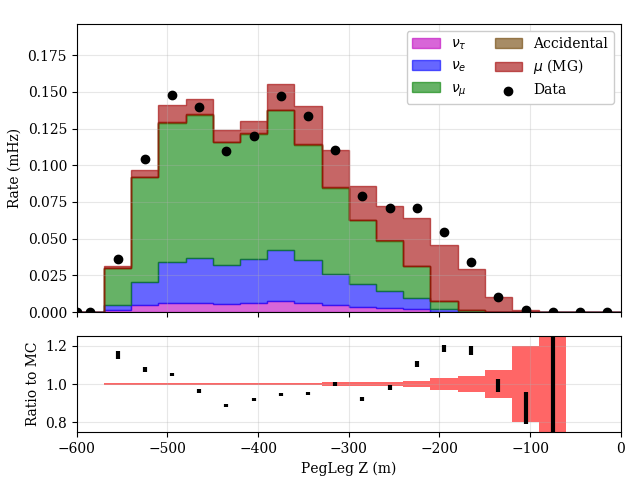
\includegraphics[width=0.6\linewidth]{L7_reco_z.png}
\caption{The reconstructed Z position using PegLeg. The GRECO L7 cuts have not been applied in order to show discrepancies below the detector. Noticeable disagreement is seen around a depth of z=-450.}
\end{figure}
\end{center}

The initial plots are shown in \ref{fig:flaring_zrho}.
A significant difference is observed at a depth of around $\mathtt{Z\approx -400}$.
Checks performed with other samples have shown similar disagreeements at these depths, indicating disagreement in the ice model.
Previously unblinded oscillation samples showing this issue have not observed significant issues in the goodness-of-fit.
New ice models are underway with dedicated work to fix this region is underway.

\begin{center}
\label{fig:flaring_zrho}
\begin{figure}
	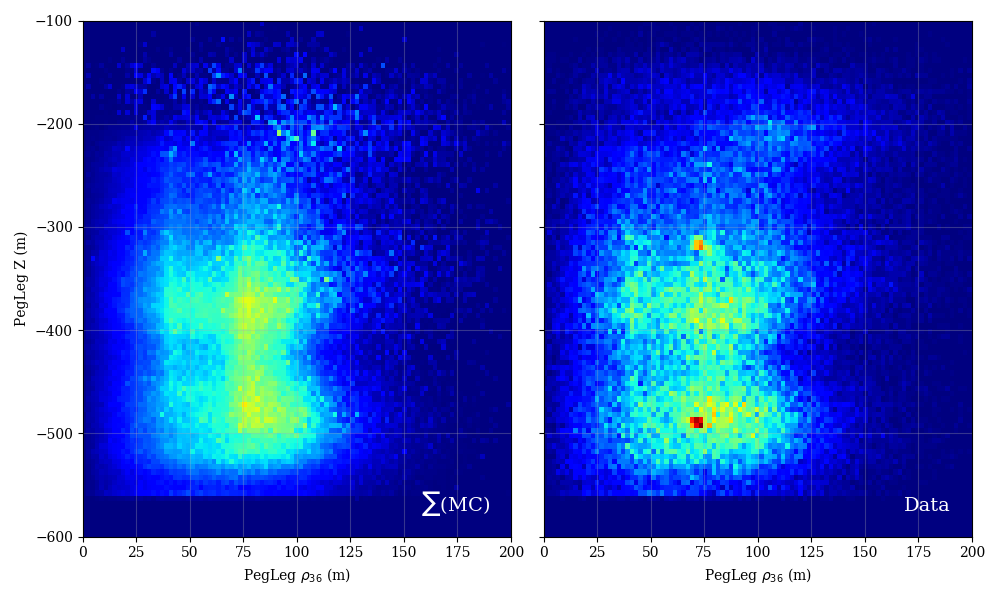
\includegraphics[width=0.9\linewidth]{pegleg_fine_z_rho.png}
\caption{The reconstructed Z position plotted against the reconstructed distance from string 36. The L7 cuts from GRECO have been removed for this plot. The colorbars in both plots have been normalized to be identical. The data and simulation show reasonable agreement except for two points in the data, near $\mathtt{\rho_{36}=75}$ at depths of -310 and -490. }
\end{figure}
\end{center}

\begin{center}
\label{fig:flaring_xy}
\begin{figure}
	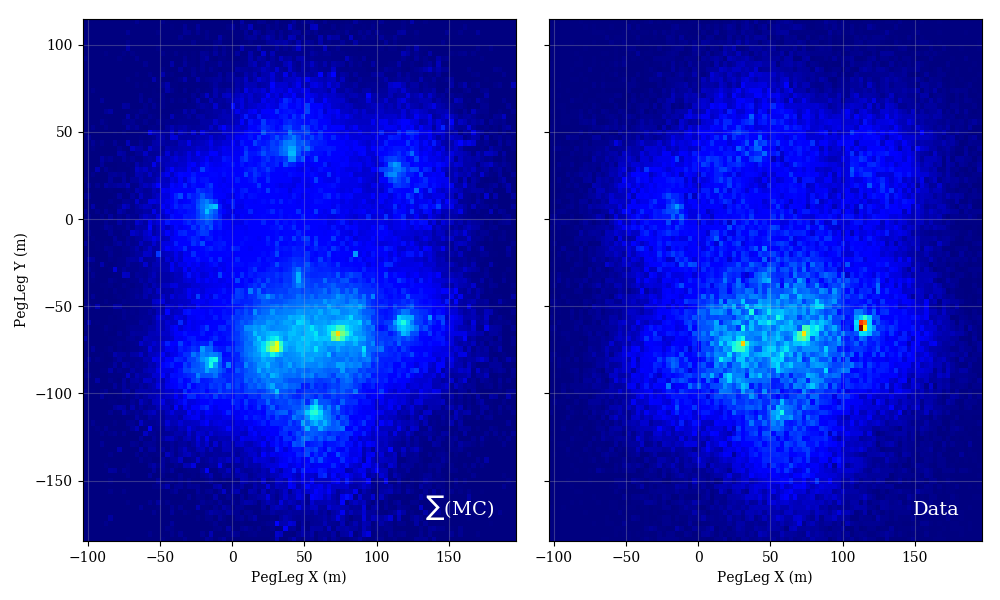
\includegraphics[width=0.9\linewidth]{pegleg_fine_x_y.png}
\caption{The reconstructed X position and Y position of events in the detector. The L7 cuts from GRECO have been removed for this plot. The colorbars in both plots have been normalized to be identical. Once again, reasonable agreement is observed in most regions, although data events have a clear excess near x=110 m, y=-60 m. This position corresponds to string 83.}
\end{figure}
\end{center}

Two-dimensional histograms of the depth and radial distance also show systematic disagreement in some regions, as shown in \ref{fig:flaring_zrho}.
These excess events appear to occur on string 83, shown in \ref{fig:flaring_xy}, indicating an effect occuring due to the DOM hardware in the detector.
Follow-up work has shown that these DOMs, known here as \textbf{flaring DOMs}, appear to spontaneously emit light for unknown reasons. 
The light output is identifiable both based on the position of the hits and the amount of charge observed in nearby DOMs.
These spurious events, first discovered in the GRECO selection, have since spawned dedicated searches to better understand spontaneous light emission from the DOMs.
A small handful of DOMs have been identified by these searches with emission times as frequent as 1 Hz \findref{internal search for flaring doms}.

The affected events may be identified based on the charge profiles. 
In particular, DOMs directly adjacent to the emitting DOM observe a significant fraction of the total charge of the event.
This may be characterized using the 'charge RMS' of the event.

\label{eqn:charge_rms}
\begin{equation}
	q_{RMS} = \frac{\sigma_q}{\sum_{hits}{q_i}}
\end{equation}

\begin{center}
\begin{figure}
	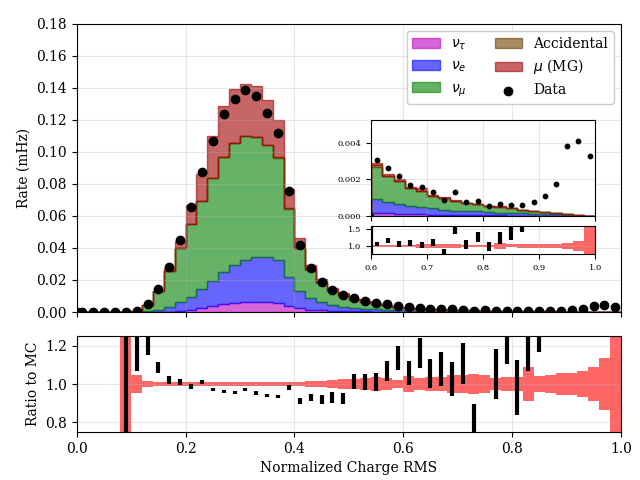
\includegraphics[width=0.9\linewidth]{L7_charge_rms_normalized.png}
\label{fig:flaring_xy}
\caption{The RMS of the charges within each event at final level. The value of the RMS is normalized using the total charge observed. The L7 cuts from GRECO are not applied here. The events with flaring DOMs cluster at high values of the charge RMS, visible in the inset.}
\end{figure}
\end{center}

This is shown in \needfig{charge rms with the excess in data}.
Events with a $\mathtt{q_{RMS}}>0.85$ are removed from the analysis, removing the most obvious spurious events. 
A total of \unsure{find the number removed by the charge rms cut in data} events are removed from the GRECO data, resulting in a total reduction of \unsure{percent reduction in number of data events}\%.
The removal of these events in data and simulation does not significantly impact the goodness-of-fit of the sample due to the low event rates involved.

\label{subsubsec:bedrock}
\subsubsection{Simulation of Bedrock}
Additional disagreement was observed in the reconstructed Z position.
Near the bottom of the detector, a clear excess of events in data indicated a mismodeling in the simulation.
This disagreement increased below the detector, shown in \needfig{reco z distribution showing disagreement with data}.
Notable disagreement was also discovered in the reconstructed energy, shown in \needfig{reco energy up to a tev showing the disagreement due to bedrock}.
Events interacting below the detector may have significantly higher energies than the reconstructed energy due to the lack of instrumentation, indicating a possible connection between these two discoveries\improvement{awkward line connecting the disagreement in recoz to high reco energy}.

In the GRECO selection, events with energies above 1 TeV are modeled using NuGen simulation in order to account for events not properly simulated in the GENIE generator.
Previous investigations have shown that the two generators use similar models of the cross-section and return similar event rates at low levels.
Still, the events from the NuGen generator were shown to make up a significant fraction of the high energy tail in the GRECO sample.
These events were therefore checked for potential issues.

The NuGen and GENIE simulated event samples are used in the GRECO analyses in non-overlapping phase spaces.
The simulations do include overlapping regions, however.
For the purposes of testing, the full sample of GENIE and NuGen events were compared in true and reconstucted energy and Z position.
Initial work comparing the overlapping energy range of NuGen and GENIE events contained within the DeepCore fiducial volume showed little apparent disagreement.

Removing the constraint on the event containment, however, led to the discovery shown in \needfig{reco z of overlapping events in nugen and genie showing the bedrock problems}.
The two generators show broad agreement until a depth of approximately -830 meters, corresponding to the interface between the Antarctic glacier and the underlying bedrock.
The difference is visible in the overlapping energy range of 100 GeV to 1 TeV.

Further checks discovered the issue in IceCube's implementation of the GENIE generator.
When calculating the interaction probability for the neutrino interactions, the density of material is included.
In the implementation of GENIE previously used by the IceCube collaboration, events were assumed to occur solely within or near the fiducial volume of DeepCore due to the low energies involved.
The bedrock was therefore deemed unnecessary and not implmented in favor of assuming a uniform density of ice throughout the simulation volume.
During initial implementation, the GENIE generator was planned for use up to 100 GeV due to technical limitations. 
Later work expanded this range up to 1 TeV with future work ongoing to push toward 10 TeV.
The problems with the bedrock were mistakenly overlooked during the upgrades of the generator, leading to the systematic disagreement shown in \needfig{reference the reco z plot showing bedrock issues again}.

The bedrock has been properly included in both the NuGen generator as well as the PROPOSAL module for propagating the charged leptons.
GENIE events therefore suffer solely from an incorrect interaction probability due to the discovered bug.
The density of interaction medium enters as a linear term in the interaction probability, indicating that a correction of the form $\mathtt{\rho_{rock}/\rho_{ice}}$ is sufficient to correct the Monte Carlo.
The fixed distributions in energy and zenith are shown in \needfig{energy and z distributions after reweighting genie bedrock events}.

In order to limit other potential issues from the bedrock, the analysis space was further limited, removing events both at higher energies ($\mathtt{E_{reco}>56 GeV}$) and those reconstructing at or below the bottom of the detector ($\mathtt{Z_{reco}\leq-500}$).
These cuts significantly reduce the size of the sample by reducing the high energy events included at final level. 
These changes have some impact on the expected sensitivity, but were deemed necessary to minimize the potential impact of systematics issues associated with the NuGen sample and, more broadly, limitations in the simulated event samples interacting below the detector.

\improvement{these updates with event rates should be lines on a data/mc rate table in the selection section.}

\label{subsubsec:final_blind_fits}
\subsubsection{Updated Results}
After the removal of the flaring DOM events, the correction of bedrock events, and the elimination of the charge in the PegLeg fit, a new blind fit was performed and the goodness-of-fit was again tested.
The resulting $\chi^2_{FS}$ for the charged-current only and neutral-current + charged-current fits were 127.095 and 127.623 respectively.
One thousand trials were run for each fit using the updated sample, yielding estimates of the probability density function shown in \needfig{PDFs for gof}.
The data is well-described by the systematics set, with a pvalue of approximately 57\% for both fits.

The final value of the systematics, plotted in \needfig{final systematics best-fits}, are within 1$\mathtt{\sigma}$ of the expectation at the best-fit points.
Many systematics were expected to be determined primarily from the data instead of from priors. 
\needfig{trials systematics distributions} shows the expected values of each systematic for 1000 trials.
The shaded band shows the assumed 1$\mathtt{\sigma}$ prior range for each of the parameters, if present.

\improvement{no idea wtf to write. its all boring stuff that's just a woooo yay it works}


\label{section:tau_results}
\section{Results from the Search for Appearance}



\label{section:other_measurements}
\section{Complementary Measurements from This Analysis}

\label{subsec:oscil_results}
\subsection{Oscillation Parameters}
Thanks to significant contributions from others \findref{future reference to martin, elim's theses}, dedicated measurements of the atmospheric mixing parameters have also been performed using the GRECO selection.
In these measurements, the value of $\mathtt{N_{\nu_\tau}}$ remains fixed to unity.
The derived results are therefore directly comparable to results from other oscillation experiments.

\label{subsubsec:disappearance_results}
\subsubsection{$\nu_\mu$ Disappearance Results}
Using similar tools as the appearance analysis, a complementary search for $\mathtt{\nu_\mu}$ disappearance was performed \findref{elim's thesis}.
The measurement of the disappearance parameters, $\mathtt{\Delta m^2_{3j}}$ and $\mathtt{\theta_{23}}$, used an identical choice of binning and systematics set as the appearance search described above.
The $\chi^2_{FS}$ statistic was found by minimization with the iMinuit package \findref{iminuit} across a grid of values arranged linearly in $\mathtt{\Delta m^2_{3j}}$ and $\mathtt{sin^2\theta_{23}}$ covering both octants.
At each point, the disappearance parameters were fixed during minimization.
Both the normal and inverted ordering are tested separately.

The result is shown in \needfig{elim's result!} with comparisons to previous atmospheric oscillation measurements by IceCube \findref{icecube 2017 result}, Super-Kamiokande \findref{superk 2015 oscillation result} and the MINOS experiment \findref{minos oscillation with atm}.
Results from accelerator measurements are shown from the $\mathtt{NO\nu A}$ \findref{nova oscillation} and T2K \findref{t2k oscillation result} experiments.
All results show the 90\% contour around the best-fit point.
The GRECO result mildly prefers the normal ordering and the second octant, although maximal mixing ($\mathtt{sin^2\theta_{23}=0.5}$ is well within the best-fit contours.

The GRECO result improves upon the most recent IceCube result significantly, particularly in the measurement of the mass splitting.
Both results are statistically consistent with one another, although the GRECO result perfers a larger mass splitting than the previous result.
Global fits, which prefer a value of the mass splitting of $\mathtt{2.494^{+0.033}_{-0.031}}$ as of the time of this writing \findref{nufit 3.2}, favor the new GRECO result over the previous IceCube result.

Precise measurements of the atmospheric mixing angle continue to elude us, however.
While the GRECO result provides competive constraints on the mixing angle, no significant improvement is observed.

\label{subsubsec:nmo_results}
\subsubsection{Mass Ordering}
In order to quantify the preference for the mass ordering, a dedicated measurement using the GRECO sample was performed \findref{martin's thesis}.
This measurement included numerous differences relative to the appearance and disappearance measurements.
Only upgoing reconstructed GRECO events were included, although the energy range was extended to 3-100 GeV.
All simulation templates were smoothed during the analysis using a dedicated implementation of the kernal density estimation technique implemented in the C++ programming language \findref{martin's kdes from the aachen group. who did that?}.
This code, unlike the SciPy KDE implementation used in \ref{sec:kde_filtering}, includes functionality for weighted event samples and variable bandwidth estimation.

The systematics set used in the mass ordering analysis was identical to that of the disappearance measurement, with the value of $\mathtt{N_{\nu_\tau}}$ fixed to unity.
Systematics included in the mass ordering measurement were applied using a parallel branch of the OscFit code used in the appearance measurement.

Statistical uncertainties arising from the simulation statistics were estimated using a bootstrapping technique included in the KDE implementation.
The test statistic used in the mass ordering measurement was defined to be the numerical convolution between the Poissonian uncertainty due to the expected event count and a Gaussian model of the bootstrapped Monte Carlo statistical uncertainty.

Unlike the appearance and disappearance measurements, the neutrino mass ordering is not a continuous parameter. 
The calculation of a final significance proceeds following the method described in \findref{pingu paper and/or pisa paper describing nmo measurement}, a full description of which is beyond the scope of this work.
Using GRECO events, a good fit is obtained at the best-fit point with a pvalue of approximately 80\%.
Using the cited technique, a weak preference for the normal mass ordering is found at approximately 0.3$\mathtt{\sigma}$ \unsure{Need martin's final result!}

\label{subsec:syst_constraints}
\section{New Constraints on Detector Systematics}
The statistics available in the GRECO dataset provide a unique chance to derive new constraints on systematic variables.
For each of the parametrized detector systematics, a scan was performed to evaluate constraints from the dataset.
In all cases, the value of $\mathtt{N_{\nu_\tau}}$ remained fixed to unity.
The results of these scans are shown in \needfig{chi2 scans of the detector systematics to show greco constraints on domeff, holeice, hifwd, absorption, and scattering}.

These new constraints imply new, tighter limits derived from fits to the detector data.
They do have limitations, however.
During the parametrization process, all systematics were assumed to be uncorrelated, which is unlikely to be the case in practice.
The DOM efficiency and absorption properties in the ice are known to have correlations in dedicated calibration work in the detector, for example.
These correlations are included in the prior uncertainties for each parameter.
Although

Each also assumes an accurate modeling of the effects in question.
All effects are assumed to equally apply to the entire detector.
Bulk changes of the properties associated with each systematic are assumed to be more important than the spread of uncertainties for each DOM (DOM efficiency, hole ice parameters) or layer in the ice (absorption, scattering).
This assumption indicates limited insight may be gained.
Testing the properties for each DOM is unlikely to be within the statistical reach of any dataset in the foreseeable future given the number of DOMs in the detector.

The new constraints from GRECO demonstrate significant power in the dataset to identify new effects like those discussed in \ref{subsec:blind_fits}.
The dataset provides the collaboration with a novel set of low energy events sensitive to evaluate detector properties.
These new constraints may be used in future analyses to limit systematic uncertainties affecting other measurements.

\label{subsec:implications}
\subsection{Implications and Future Work}
There exist various ways to interpret the value of $\mathtt{N_{\nu_\tau}}$. 
The value of the tau neutrino normalizations in the exclusive and inclusive channels \improvement{change cc and nc+cc to exclusive and inclusive respectively?} are both consistent with the expected value of 1.0.
The standard 3-flavor oscillation model is not strongly disfavored from the GRECO oscillation result.
The current result does, however, provide some tension with the most recent exclusive result from Super-Kamiokande \findref{superk result}, which reported $\mathtt{1.47\pm0.32}$. 
The GRECO and Super-Kamiokande inclusive results differ by approximately 1.8$\mathtt{\sigma}$, assuming the total uncertainties are added in quadrature.
In practice, various systematics, including the atmospheric mixing angle and mass splitting, are likely correlated between the analyses, implying approximately 2$\mathtt{\sigma}$ of tension between the two results.

Assuming Gaussian uncertainties for the two results, the simple weighted average can be calculated in order to estimate the expectation from a combined fit.
This value, $\mathtt{1.06\pm0.22}$, shows remarkable agreement with the expected value of 1.0, favoring the standard 3-flavor mixing matrix with large uncertainties.
The OPERA value \findref{opera result}, which strongly excludes the no-appearance hypothesis but little else, has a negligible effect on this average.

This analysis, like previous oscillation analyses produced by IceCube, has limitations.
The GRECO selection includes only three years of detector data.
The runs of data from those three years are selected using strict criteria that explicitly excludes non-standard runs, including those that are ended prematurely.
These short runs are often otherwise unremarkable, butmake up a significant fraction of the uptime of the detector in these years and are potentially useful for analysis.
The addition of these runs may increase the total number of events in the GRECO sample by up to 15\% \unsure{what's the livetime increase from loosing the GRL?}.
The addition of these events presents a simple way to improve the existing result on relatively short timescales.

The three years of data may also be extended in other ways.
The data was originally collected between April 2012 and May 2015 \unsure{check the run dates}.
Since the beginning of this work, additional years of detector data have been collected and are awaiting analysis.
These additional years of data were not included due to calibration changes in the IC86-5 season which may lead to disagreement between years.
These updated calibrations have since been applied to the earlier years of detector data as well, leading to a self-consistent dataset of approximately 7 years.

The analysis of these events requires a number of upgrades to the simulation which are ongoing at the time of this work.
New efforts are underway updating the simulated SPE templates (\ref{subsubsec:charge_templates}) to better describe the charge profile observed in the detector.
These new templates are fit to detector data for each DOM and are updated for each year, although the year-to-year variations have proven to be small.
New signal and background simulation is therefore necessary to incorporate these upgrades.
The new simulations are underway, with completion and verification expected within the coming year.
If the new sets show good agreement with data, charge information may be reintroduced to the reconstruction, potentially leading to improvements in the reconstructed resolution of events.

The current GRECO selection was the first oscillation analysis in IceCube to succesfully use simulated atmospheric muon background events at analysis level.
The simulated livetime is too limited, at 10 months, to allow for precision measurements using the additional years of data.
While the GRECO selection is efficient at rejecting these simulated muons, additional simulation efforts require vast computational resources.
Future analyses will require significantly larger muon datasets in order to adequately describe backgrounds.
The production of additional events for these analyses will require nearly a factor of 9 more events to reach parity between the expected number of muon events in 7 years of data and the raw Monte Carlo statistics.
If only the standard simulation methods are used, this will require about 1.5 years worth of production time.
While the new sets would include muon bundles, a feature not present during production of this work, the sets may still be limited outside of the DeepCore fiducial volume.

To remedy this situation, work is ongoing to further develop and standardize the work described in \ref{sec:kde_filtering}. 
That effort has been shown to yield significant improvements to the production time of MuonGun simulation, with a typical speedup of 3-4x for muons produced for the GRECO selection when using no DOM oversizing.
This can improve to factors of 15-20x if using a DOM oversizing factor of 3.
This may be a viable option for the production of various systematics sets in order to speed the production of background events.
Additional improvements to the simulation efficiency are possible and will undoubtedly be investigated in the near future.
Even using the improvements described here, however, large muon sets are, for the first time, viable as background models in IceCube oscillation analyses.

Improvements are not only possible in the background simulation, however.
Investigations described in \ref{subsubsec:bedrock} have spawned discussions of the limitations of the current GENIE generatior production scheme.
While GENIE was originally planned to be used solely for very low energy oscillation analyses, the dawn of new event selections such as GRECO spanning wider energy ranges can lead to notable disagreement traceable to the generation scheme.
To better describe the detector, GENIE generation must be exampled to identify unsimulated phase space necessary for further analyses.
The simulation of events below the detector, in both the GENIE generator as well as in future MuonGun background simulations, must be given priority in order to explain the events occuring at the bottom or below the IceCube detector.



